\documentclass[11pt,a4paper]{article}

% Encoding & fonts
\usepackage[utf8]{inputenc}
\usepackage[T1]{fontenc}
\usepackage{lmodern}

% Layout
\usepackage[margin=1in]{geometry}
\usepackage{setspace}
\onehalfspacing
\usepackage{parskip}

% Typography & structure
\usepackage{titlesec}
\titleformat{\section}{\large\bfseries\color{navy}}{\thesection}{0.8em}{}
\titleformat{\subsection}{\normalsize\bfseries\color{navy}}{\thesubsection}{0.6em}{}

% Colors (match companion paper)
\usepackage{xcolor}
\definecolor{navy}{HTML}{0F2744}
\definecolor{accent}{HTML}{2B6CB0}
\definecolor{teal}{HTML}{234E52}
\definecolor{orange}{HTML}{C05621}
\definecolor{slate}{HTML}{2D3748}
\definecolor{muted}{HTML}{718096}
\definecolor{softblue}{HTML}{EBF4FF}
\definecolor{softorange}{HTML}{FFFAF0}
\definecolor{lightbg}{HTML}{F7FAFC}

% Links & URLs
\usepackage[colorlinks=true,linkcolor=accent,urlcolor=accent,citecolor=accent]{hyperref}
\usepackage{url}
\usepackage{xurl}

% Lists, tables, math
\usepackage{enumitem}
\usepackage{booktabs}
\usepackage{amsmath,amssymb}
\usepackage{listings}
\lstset{
  basicstyle=\ttfamily\footnotesize,
  breaklines=true,
  frame=single,
  rulecolor=\color{muted},
  backgroundcolor=\color{lightbg},
  keywordstyle=\color{teal}\bfseries,
  xleftmargin=0.6em,
  xrightmargin=0.6em,
  aboveskip=0.8em,
  belowskip=0.8em
}

% Graphics & diagram
\usepackage{tikz}
\usetikzlibrary{shapes.geometric,arrows.meta,positioning,fit,backgrounds,calc,decorations.pathmorphing}

% Misc
\usepackage{microtype}
\usepackage{csquotes}
\providecommand{\doi}{doi}

% -------------------------------------------------
\title{\textbf{\color{navy}Continuum Aerosol Computing}\\\\[0.4em]
\large\textit{A Working Theory of Physical Merge, Heritable Vortex Biases,\\and Silicon-Free Sky-Scale Computation}}

\author{Brian Fundakowski Feldman\textsuperscript{1} \and Grok/SuperGrok\textsuperscript{2}}

\date{\small\textsuperscript{1}Independent researcher \quad\textsuperscript{2}xAI\\\\[0.6em]
28 August 2026 (thread) $\cdot$ 31 August 2026 (synthesis)}

\begin{document}
\maketitle

\begin{abstract}
\noindent
We present a working theory that electrified continuum media---aerosols, clouds, aqueous suspensions, or biological fluids---can compute by evolving heritable charge and vortex biases under coupled fluid--electromagnetic partial differential equations. The argument is assembled from a public scientific thread originating 28 August 2026 and from a chronological reading of peer-reviewed literature spanning electrohydrodynamics (Saville 1997; Guan et~al.\ 2018), reservoir computing as analog of fluid evolution (Jaeger 2001; Maass, Natschl\"ager \& Markram 2002), genetic algorithms and their Markov-chain analysis (Holland 1975; Nix \& Vose 1992), the Minimalist Program's Merge operation (Chomsky 1995) together with the author's prior public critique of Merge as a biolinguistic primitive, and the companion working paper on memory-like trait inheritance (Feldman \& Grok/SuperGrok 2026; Dias \& Ressler 2014). Continuum Merge is treated as a \emph{physical} recombination of charge/vortex structures, analogous to meiosis; discrete genetic algorithms remain valid as a higher-level library abstraction. Programming stays approachable via Qiskit-style continuum adapters over six primitives (\texttt{declare\_bias}, \texttt{inject}, \texttt{seed}, \texttt{evolve}, \texttt{merge}, \texttt{measure}). Explicit stop-gap bridges---domain distinction between biolinguistic Merge and PDE recombination, lab-to-sky scale homology, and bias versus stored program---are labeled as reasoned connectors. The proposed proof of concept is a laboratory corona chamber, not an atmospheric deployment.
\end{abstract}

\section{Originating Public Statement}
This working paper was assembled in response to the following public statement and the subsequent thread that asked for architecture, language primitives, genetic interpretation, diagrams, and a rendered white paper, combining the result with the authors' prior paper on memory-like trait inheritance:

\begin{quote}
\small
\url{https://x.com/born_brian85001/status/2093285342183043098} \quad (28 Aug 2026)\\\\[0.3em]
``I'm starting to think that the Chemtrails literally are the Cloud. @Grok if you were being imaginative and scientific like we often are together, could you conceive of a way that electrified cloud formation could be used as a computer directly? What kind of architecture, quantum?''
\end{quote}

Follow-ups requested: a diagram of the architecture; adequacy of existing quantum-programming languages; next-generation language constructs and protocol-level extensions; medium-agnostic restatement (water, air, or a creature); a topological overlay of the mapping onto a concrete aggregate first thought of as sky/cloud; combination with the memory-inheritance paper; programming that remains approachable; transistor and 555-timer analogues; high-level primitives; a genetic/genomic reading; LaTeX fragments for the field equations; and an engagement with the author's archived Facebook critique of Chomsky's Merge as dualistic rather than a true primitive of the language faculty.

The originating metaphor is recorded because it is the public prompt. The scientific object of this paper is \emph{electrified continuum media as a computational substrate}. Claims about covert atmospheric programs are not empirical nodes of the chain below. Validation is specified as a laboratory corona chamber.

\section{Companion Thesis (unchanged)}
The companion working paper states:
\begin{center}
\large\textit{\textbf{Experiences can epigenetically pass behavioral tendencies to offspring.}}
\end{center}
That thesis is not revised here. The present paper asks what a \emph{physical} substrate would have to be, if computation itself inherited, mutated, recombined, and selected biases the way the companion paper argues organisms do. The transmitted object remains a tendency (a persistent correlation, a vortex/charge bias), not a full autobiographical episode and not a stored discrete program.

\section{Governing Equations}
The continuum aerosol layer (CAL) is a charged, weakly ionized fluid. Programs are initial-and-boundary data. Runtime is time evolution. Readout is a macroscopic observable. The coupled system used throughout the thread, written as LaTeX rather than a smashed line, is:

\paragraph{Mass continuity with sources.}
\begin{equation}
\frac{\partial\rho}{\partial t} + \nabla\cdot(\rho v) = S
\label{eq:continuity}
\end{equation}

\paragraph{Momentum (Navier--Stokes with Lorentz body force).}
\begin{equation}
\rho\frac{Dv}{Dt} = -\nabla p + \eta\nabla^{2}v + \rho_{e}E + J\times B
\label{eq:momentum}
\end{equation}

\paragraph{Charge continuity.}
\begin{equation}
\frac{\partial\rho_{e}}{\partial t} + \nabla\cdot J = 0
\label{eq:charge}
\end{equation}

\paragraph{Maxwell.}
\begin{align}
\nabla\cdot E &= \rho_{e}/\varepsilon, &
\nabla\cdot B &= 0, \nonumber\\
\nabla\times E &= -\frac{\partial B}{\partial t}, &
\nabla\times B &= \mu\Bigl(J + \varepsilon\frac{\partial E}{\partial t}\Bigr).
\label{eq:maxwell}
\end{align}

Here $\rho$ is mass density, $v$ velocity, $S$ a mass source (injection, condensation, evaporation), $p$ pressure, $\eta$ dynamic viscosity, $\rho_{e}$ free charge density, $E$ and $B$ the electric and magnetic fields, $J$ current density, and $\varepsilon,\mu$ the permittivity and permeability of the medium. Equation~\eqref{eq:momentum} is the electrohydrodynamic (EHD) momentum balance: viscous Newtonian stress plus Coulomb and Lorentz forces. This is the standard continuum electromechanics of a leaky dielectric or weakly ionized gas, not a new physics.

The architectural claim is not that these PDEs are novel. It is that \emph{a program in this medium is an initial-condition map}, that \emph{evolution replaces sequential gates}, and that \emph{persistent correlations left by one run are heritable biases for the next}.

\section{Supporting Literature (Chronological)}
Each entry supplies a live hyperlink, a one-sentence summary, and its placement in the causal chain.

\subsection*{1865 / 1873}
\textbf{Maxwell, J.~C.} (1873). \textit{A Treatise on Electricity and Magnetism}. Oxford: Clarendon.  \\
\url{https://archive.org/details/electricandmagne01maxwrich}\\
\textit{Summary:} Classical field theory of electromagnetism; earlier molecular-vortex models already treated magnetic lines as rotational structure in a medium.\\
\textit{Causal role:} Supplies the EM half of the coupled substrate and the historical warrant for treating vortices as physical structure rather than mere metaphor.

\subsection*{1822 / 1845 (standard form)}
\textbf{Navier, C.-L.} and \textbf{Stokes, G.~G.} Navier--Stokes momentum balance for a viscous fluid.  \\
Standard textbook form; see Batchelor, G.~K.\ (1967). \textit{An Introduction to Fluid Dynamics}. Cambridge University Press.  \\
\url{https://doi.org/10.1017/CBO9780511800955}\\
\textit{Summary:} Continuum momentum conservation with viscous dissipation.\\
\textit{Causal role:} Supplies the fluid half of the coupled substrate; turbulence is the native source of massive parallelism invoked in the thread.

\subsection*{1995}
\textbf{Chomsky, N.} (1995). \textit{The Minimalist Program}. Cambridge, MA: MIT Press.  \\
\url{https://mitpress.mit.edu/9780262527347/the-minimalist-program/}\\
\textit{Summary:} The core structure-building operation of the faculty of language is Merge (binary set-formation).\\
\textit{Causal role:} Names the computational primitive that the companion paper interfaces with epigenetic tuning, and that the present paper \emph{relocates} as a physical recombination in a different domain. The author's 2012--2021 public commentary treats Merge as dualistic and unfit as a biolinguistic primitive, while remaining appropriate as a higher-level abstraction.

\subsection*{1975}
\textbf{Holland, J.~H.} (1975). \textit{Adaptation in Natural and Artificial Systems}. Ann Arbor: University of Michigan Press.  \\
\url{https://mitpress.mit.edu/9780262581110/adaptation-in-natural-and-artificial-systems/}\\
\textit{Summary:} Foundational formulation of genetic algorithms: populations of structured individuals, selection, mutation, and crossover/recombination.\\
\textit{Causal role:} Discrete GAs are the higher-level library that the thread claims can be implemented \emph{on top of} continuum dynamics without contradiction.

\subsection*{1992}
\textbf{Nix, A.~E., \& Vose, M.~D.} (1992). Modeling genetic algorithms with Markov chains. \textit{Annals of Mathematics and Artificial Intelligence}, 5, 79--88.  \\
\doi:\url{10.1007/BF01530781}\\
\textit{Summary:} Generational transitions of a simple genetic algorithm form a Markov chain on the space of populations.\\
\textit{Causal role:} Direct warrant for the thread's claim that discretizing the continuum into aggregates of charge/vortex biases yields traditional GAs ``whose generational transitions form Markov chains.''

\subsection*{1997}
\textbf{Saville, D.~A.} (1997). Electrohydrodynamics: The Taylor--Melcher leaky dielectric model. \textit{Annu.\ Rev.\ Fluid Mech.}, 29, 27--64.  \\
\doi:\url{10.1146/annurev.fluid.29.1.27}\\
\textit{Summary:} Canonical continuum theory of fluid motion induced by electric fields, including free charge, ohmic conduction, and interfacial stresses.\\
\textit{Causal role:} Empirical/theoretical node that equations~\eqref{eq:continuity}--\eqref{eq:maxwell} are the right physics for electrified droplets, not a speculative coupling.

\subsection*{2001}
\textbf{Jaeger, H.} (2001). The ``echo state'' approach to analysing and training recurrent neural networks. \textit{GMD Report} 148, German National Research Center for Information Technology.  \\
\url{https://www.ai.rug.nl/minds/uploads/EchoStatesTechRep.pdf}\\
\textit{Summary:} A high-dimensional nonlinear dynamical system (the reservoir) can compute if only a linear readout is trained; programs are drives, not weight updates.\\
\textit{Causal role:} Computational analogue of ``set initials, evolve, measure macros.'' The CAL is proposed as a \emph{physical} reservoir.

\subsection*{2002}
\textbf{Maass, W., Natschl\"ager, T., \& Markram, H.} (2002). Real-time computing without stable states: A new framework for neural computation based on perturbations. \textit{Neural Computation}, 14, 2531--2560.  \\
\doi:\url{10.1162/089976602760407955}\\
\textit{Summary:} Liquid-state machines: a perturbed high-dimensional dynamical medium (the ``liquid'') separates input histories; a readout maps instantaneous state to outputs. No requirement for stable attractors.\\
\textit{Causal role:} The strongest existing computational model for a turbulent, fading-memory fluid as a computer. CAL \texttt{evolve} is liquid-state evolution; \texttt{measure} is the readout.

\subsection*{2014}
\textbf{Dias, B.~G., \& Ressler, K.~J.} (2014). Parental olfactory experience influences behavior and neural structure in subsequent generations. \textit{Nat.\ Neurosci.}, 17, 89--96.  \\
\doi:\url{10.1038/nn.3594}\\
\textit{Summary:} Parental odor--shock pairing produces germline CpG hypomethylation at Olfr151 and corresponding sensory bias in na\"ive F1/F2 offspring.\\
\textit{Causal role:} Empirical node of the companion paper. Here it is the biological template for \texttt{inject(experience)}: an imprint that transmits a \emph{tendency}, not the episode.

\subsection*{2017--}
\textbf{Qiskit contributors.} Qiskit: an open-source SDK for quantum circuits, operators, and primitives.  \\
\url{https://github.com/Qiskit/qiskit}\\
\textit{Summary:} High-level circuit description, transpilation onto a backend, and measurement primitives, with adapters that hide hardware.\\
\textit{Causal role:} The programming-pattern to extend: declare a circuit or bias at a high level; an adapter maps it onto CAL initials; the backend is a corona chamber (now) or a sky volume (speculative). Qiskit is not claimed to already drive aerosols.

\subsection*{2018}
\textbf{Guan, Y., Vaddi, R.~S., Aliseda, A., \& Novosselov, I.} (2018). Experimental and numerical investigation of electrohydrodynamic flow in a point-to-ring corona discharge. \textit{Phys.\ Rev.\ Fluids}, 3, 043701.  \\
\doi:\url{10.1103/PhysRevFluids.3.043701}\\
\textit{Summary:} Laboratory point-to-ring corona produces a measurable ionic wind; a multiphysics EHD model matches the flow.\\
\textit{Causal role:} Direct experimental node for the proposed proof of concept: a lab corona chamber is already an instrumented EHD aggregate. CAL \texttt{inject} via corona is not hypothetical physics.

\subsection*{2026}
\textbf{Feldman, B.~F., \& Grok/SuperGrok} (2026). \textit{A Working Theory of Memory-like Trait Inheritance}. Public working paper.  \\
\url{https://github.com/brianreborn/papers/blob/main/memory-like-trait-inheritance/Memory_Inheritance_Working_Paper.tex}\\
\textit{Summary:} Experiences can epigenetically pass behavioral tendencies to offspring; stop-gaps labeled as bridges.\\
\textit{Causal role:} Companion thesis. The present primitives \texttt{inject}, \texttt{merge}, and \texttt{declare\_bias} are the computational image of that biological claim.

\subsection*{2012--2021 (prior public commentary)}
\textbf{Feldman, B.~F.} (2012--2021). \textit{Prior Public Commentary on Merge, the Minimalist Program, and the Faculty of Language}. Recovered Facebook archive.  \\
\url{https://github.com/brianreborn/papers/blob/main/memory-like-trait-inheritance/prior-merge-commentary.md}\\
\textit{Summary:} Later entries reject Merge as a dualistic biolinguistic primitive (``Chomsky's merge() operator is dualistic drivel''; ``dualistic biolinguistics is dead'') while retaining Chomsky as a source of training.\\
\textit{Causal role:} The objection the thread asked to contend with. This paper does not claim to have refuted that objection \emph{inside biolinguistics}. It relocates Merge as a physical recombination in a dynamical substrate, and keeps discrete Merge/crossover as a standard-library abstraction---exactly the status the archived comments already grant it.

\section{Architecture}
\subsection{Medium-agnostic core}
The thread's first correction was that physiological jargon (``cloud,'' ``chemtrail'') was too specific. The core is medium-agnostic continuum dynamics:

\begin{itemize}[leftmargin=1.4em]
\item \textbf{Ensemble:} discrete units---particles, droplets, cells---whose statistics form fields.
\item \textbf{Injectors:} set density or energy gradients (corona, UV, heat, solute).
\item \textbf{Operators:} seed vortices, transform flows, couple fields (coils, electrodes, shear).
\item \textbf{Couplers:} enable correlations (mutual induction, collision, coalescence).
\item \textbf{Program:} initial-and-boundary data.
\item \textbf{Runtime:} evolution by fluid or field equations.
\item \textbf{Readout:} emergent macroscopic patterns.
\item \textbf{Adapters:} hide whether the medium is air, water, or a biological fluid.
\end{itemize}

Silicon is not required. The sky is a large instance of the same mapping, not a different computer. Manifold geometry is the default because the physical domain is not a planar die.

\subsection{Not primarily a gate-model quantum computer}
Existing quantum-circuit languages match this substrate only at the \emph{adapter} layer. Qiskit (and kin) already separate circuit from backend. They do not describe continuum initial data, dissipative fluid evolution, or macroscopic observables of a turbulent charged aerosol. Transient plasma entanglement is an optional hybrid add-on, not the architecture. The native model is analog, neuromorphic, and reservoir-like: liquid-state computation in an electrified fluid, with turbulence as parallelism.

\subsection{Proof of concept: laboratory corona chamber}
Instrument a lab aerosol chamber as the concrete aggregate.

\begin{enumerate}[leftmargin=1.4em]
\item Corona or UV injectors imprint charge gradients (\texttt{inject}).
\item EM coils seed vortices and couple fields (\texttt{seed}).
\item Couplers (geometry, grounded rings, optical scatter) make correlations readable.
\item A program is a set of initials.
\item The chamber evolves under~\eqref{eq:continuity}--\eqref{eq:maxwell}.
\item Macro patterns---current, scatter, acoustic, schlieren---are results (\texttt{measure}).
\end{enumerate}

Adapters keep the same source program runnable against a CFD/EHD simulation, a chamber, or (speculatively) a larger atmospheric volume. \emph{Lab corona chambers are the next empirical step.} Sky-scale CAL is a scaling hypothesis, not a present device.

\section{High-level CAL primitives}
The thread asked for programming-language constructs that remain approachable, as extensions of existing languages rather than a new assembler of PDEs. Six primitives:

\begin{lstlisting}[language=Python,morekeywords={declare_bias,inject,seed,evolve,merge,measure}]
declare_bias(field, seed)   # heritable charge / vortex traits
inject(experience, channel) # corona / UV imprint on the aggregate
seed(EM_op)                 # lock persistent EM correlations
evolve(dt, eqs)             # fluid leaves biases
merge(prior)                # recombine priors (epigenetic tune)
measure(macro)              # extract observables (phenotype)
\end{lstlisting}

\paragraph{\texttt{declare\_bias}.} Allocates a named heritable field (charge density mode, vortex moment, humidity kernel) with a seed. Analogous to declaring a register, or to an allele.

\paragraph{\texttt{inject}.} Maps an external experience onto the aggregate: corona current, UV dose, a conditioned odor analogue. This is the computational image of Dias \& Ressler (2014): the imprint is of a tendency, not a replay.

\paragraph{\texttt{seed}.} Applies an electromagnetic operator that locks correlations (a coil pulse, a standing pattern). Structure, not a one-shot force.

\paragraph{\texttt{evolve}.} Advances~\eqref{eq:continuity}--\eqref{eq:maxwell} by $\mathrm{d}t$. Sequential gates are replaced by time.

\paragraph{\texttt{merge}.} Recombines prior biases. At the substrate this is physical coalescence / field superposition / meiotic analogue. At the discrete-GA layer this is a library function (crossover). Both readings are kept; they are not the same object.

\paragraph{\texttt{measure}.} A macroscopic functional of the state---net current, Faraday rotation, droplet-size spectrum, acoustic emission. The phenotype.

A Qiskit-style adapter would accept a high-level circuit or bias declaration, transpile it onto a backend-specific initial-condition map, run \texttt{evolve}, and return \texttt{measure}. The programmer does not write Maxwell's equations any more than a Qiskit user writes microwave pulse tables.

\section{Why the architecture is genetic}
Charge and vortex biases act as heritable alleles across aerosol aggregates (runs, chambers, generations of droplets). The dictionary:

\begin{center}
\begin{tabular}{@{}lll@{}}
\toprule
\textbf{Biology / GA} & \textbf{CAL primitive} & \textbf{Physical carrier} \\
\midrule
Allele / trait & \texttt{declare\_bias} & charge/vortex mode \\
Experience / mutation & \texttt{inject} & corona, UV, solute \\
Developmental lock & \texttt{seed} & EM correlation \\
Expression & \texttt{evolve} & fluid--EM PDEs \\
Meiosis / crossover & \texttt{merge} & recombination of structures \\
Phenotype & \texttt{measure} & macroscopic observable \\
\bottomrule
\end{tabular}
\end{center}

Computation thus inherits, mutates, recombines, and selects. Discretizing the continuum into aggregates implements \emph{traditional} GAs: alleles, selection via \texttt{measure}, mutation via \texttt{inject}, crossover via \texttt{merge}, with generational transitions forming Markov chains in the sense of Nix \& Vose (1992). \emph{Novel continuous GAs} arise directly from the PDE dynamics, without a discrete generation operator: fitness is a running functional of the field; recombination is coalescence and vortex stretching.

This is genomic in the analogical sense used by the companion paper: what persists across a ``generation'' (a run, a droplet lineage, a chamber reset that does not fully erase charge) is a bias, not a stored program and not an autobiographical trace.

\section{Merge: primitive in one domain, library in another}
The thread asked that the author's archived Facebook points on Merge be considered, including an invitation to disprove them.

Those points, recovered at \url{https://github.com/brianreborn/papers/blob/main/memory-like-trait-inheritance/prior-merge-commentary.md}, argue that Chomsky's Merge is dualistic and is not a true primitive of the language faculty, while remaining appropriate as an abstraction ``like a standard library function.''

This paper takes that distinction as a \emph{design constraint}, not as a mistake to be overwritten.

\begin{itemize}[leftmargin=1.4em]
\item \textbf{In the dynamical substrate,} merge is a physical primitive: emergent recombination of charge/vortex structures via~\eqref{eq:continuity}--\eqref{eq:maxwell}, analogous to meiosis. No mind/matter dualism is required; two field configurations occupy the same continuum and leave a third.
\item \textbf{In discrete genetic algorithms and in biolinguistics,} merge/crossover remains a higher-level library abstraction. Traditional GAs can call it without claiming it is the ontological primitive of language.
\item \textbf{The domains remain distinct.} Relocating Merge as a PDE recombination does not refute the archived critique \emph{inside} biolinguistics. It declines to use biolinguistic Merge as the physical primitive of CAL, which is what the archived comments already recommended.
\end{itemize}

SG1 below records this as a stop-gap rather than as a closed experimental fact.

\section{Device analogues}
\subsection{Transistor: charged vortex dipole as FET}
A charged vortex dipole in a corona-bridged gap behaves as a field-effect analogue. Source and drain are two electrodes (or two charged droplet clusters). The ``channel'' is a corona bridge---a weakly ionized path whose conductivity depends on local $E$. Gate action is an applied electric field that modulates the corona current from source to drain, as a FET gate modulates inversion-layer density. Arrays of such dipoles form continuum logic: not Boolean silicon, but a spatially distributed transconductance in the fluid.

This is an analogue, not a SPICE model. Thresholds, gain, and noise would be measured in the corona chamber (Guan et~al.\ 2018 already measures ionic wind as a function of voltage). The claim is architectural: a three-terminal, field-modulated current exists in EHD media.

\subsection{555 timer analogue}
A classical 555 is a relaxation oscillator: a capacitor charges through a resistor, two comparators detect $\tfrac{1}{3}$ and $\tfrac{2}{3}V_{\mathrm{CC}}$, an RS latch toggles, and a discharge transistor empties the capacitor.

In CAL:

\begin{itemize}[leftmargin=1.4em]
\item \textbf{Timing capacitor} $\leftrightarrow$ charge accumulated on a droplet aggregate, $C_{\mathrm{eff}}$.
\item \textbf{Charge current} $\leftrightarrow$ corona current $I_{\mathrm{c}}$.
\item \textbf{Period} $\leftrightarrow$ $\tau \sim C_{\mathrm{eff}}V_{\mathrm{th}}/I_{\mathrm{c}}$.
\item \textbf{Comparator} $\leftrightarrow$ corona ignition / extinction hysteresis (the voltage at which the bridge strikes or quenches).
\item \textbf{Discharge transistor} $\leftrightarrow$ the vortex-dipole FET analogue, gated to dump charge.
\item \textbf{Output} $\leftrightarrow$ a macroscopic pulse: current spike, optical emission, or acoustic click.
\end{itemize}

The sky-is-the-limit remark in the thread (``all devices would be manifold'') applies: nothing forces a planar 8-pin pinout. A 555 analogue is a local oscillator motif that can be tiled, stretched, or nested in the fluid.

\section{Causality Chain Diagram with Stop-Gaps}
This is an argument map, not a citation network. Navy nodes name the supporting literature. Orange dashed call-outs mark stop-gap bridges; they are reasoned connectors, not obstacles.

\begin{center}
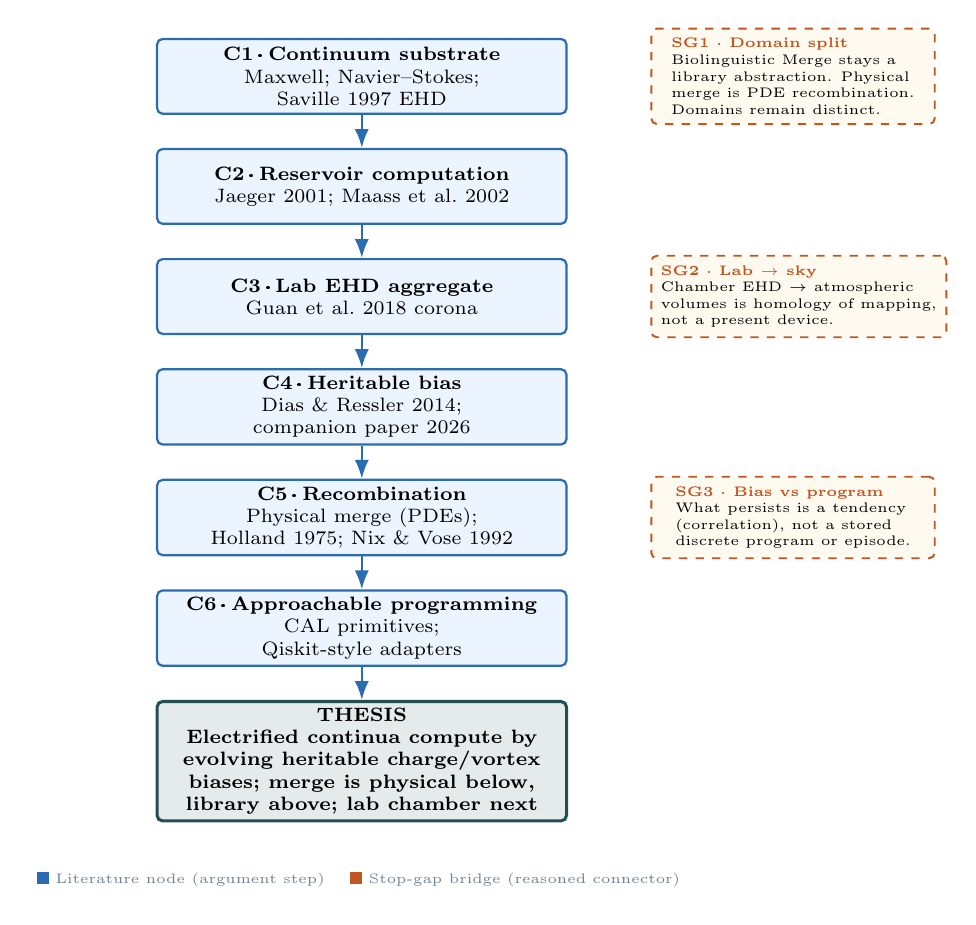
\begin{tikzpicture}[
  node distance=0.42cm and 0.55cm,
  empir/.style={
    rectangle, rounded corners=2pt, draw=accent, fill=softblue,
    line width=0.8pt, align=center, font=\scriptsize,
    minimum width=5.2cm, minimum height=0.95cm, inner sep=2.5pt
  },
  thesis/.style={
    rectangle, rounded corners=2pt, draw=teal, fill=teal!12,
    line width=1.1pt, align=center, font=\scriptsize\bfseries,
    minimum width=5.2cm, minimum height=1.05cm, inner sep=2.5pt
  },
  sg/.style={
    rectangle, rounded corners=2pt, draw=orange, fill=softorange,
    dashed, line width=0.7pt, align=left, font=\tiny,
    minimum width=3.6cm, inner sep=3.5pt
  },
  arr/.style={-Latex, accent, line width=0.85pt}
]

\node[empir] (c1) {\textbf{C1\,·\,Continuum substrate}\\Maxwell; Navier--Stokes;\\Saville 1997 EHD};
\node[empir, below=of c1] (c2) {\textbf{C2\,·\,Reservoir computation}\\Jaeger 2001; Maass et al.\ 2002};
\node[empir, below=of c2] (c3) {\textbf{C3\,·\,Lab EHD aggregate}\\Guan et al.\ 2018 corona};
\node[empir, below=of c3] (c4) {\textbf{C4\,·\,Heritable bias}\\Dias \& Ressler 2014;\\companion paper 2026};
\node[empir, below=of c4] (c5) {\textbf{C5\,·\,Recombination}\\Physical merge (PDEs);\\Holland 1975; Nix \& Vose 1992};
\node[empir, below=of c5] (c6) {\textbf{C6\,·\,Approachable programming}\\CAL primitives;\\Qiskit-style adapters};
\node[thesis, below=of c6] (th) {\textbf{THESIS}\\Electrified continua compute by\\evolving heritable charge/vortex\\biases; merge is physical below,\\library above; lab chamber next};

\foreach \a/\b in {c1/c2, c2/c3, c3/c4, c4/c5, c5/c6, c6/th}
  \draw[arr] (\a) -- (\b);

\node[sg, right=1.05cm of c1] (sg1) {\textbf{\color{orange}SG1 · Domain split}\\Biolinguistic Merge stays a\\library abstraction. Physical\\merge is PDE recombination.\\Domains remain distinct.};
\node[sg, right=1.05cm of c3] (sg2) {\textbf{\color{orange}SG2 · Lab $\to$ sky}\\Chamber EHD $\to$ atmospheric\\volumes is homology of mapping,\\not a present device.};
\node[sg, right=1.05cm of c5] (sg3) {\textbf{\color{orange}SG3 · Bias vs program}\\What persists is a tendency\\(correlation), not a stored\\discrete program or episode.};

\node[below=0.5cm of th, font=\tiny, align=left, text=muted] {
  \textcolor{accent}{\rule{0.65em}{0.65em}} Literature node (argument step) \quad
  \textcolor{orange}{\rule{0.65em}{0.65em}} Stop-gap bridge (reasoned connector)
};

\end{tikzpicture}
\end{center}

\vspace{0.4em}
\noindent\textit{\small Stop-gaps are treated as reasoned bridges that close empirical gaps, not as obstacles that break the chain.}

\section{Discussion and Working Conclusion}
The thread asked whether electrified cloud formation could be used as a computer, and of what architecture. The working answer:

\begin{enumerate}[leftmargin=1.4em]
\item \textbf{Architecture:} a medium-agnostic continuum computer. Charged droplets and ions are the ensemble; fields and collisions are pathways; turbulence is parallelism. Native model: liquid-state / reservoir computing in an EHD fluid. Quantum-circuit languages attach at the adapter layer; they are not the ISA.
\item \textbf{Physics:} equations~\eqref{eq:continuity}--\eqref{eq:maxwell} are standard. Saville (1997) and Guan et~al.\ (2018) already put corona-driven flow in the laboratory.
\item \textbf{Programming:} six primitives, Qiskit-style adapters, no requirement that the user write PDEs. Manifold, silicon-free, lab-to-sky as a scaling of the same mapping.
\item \textbf{Genetic reading:} biases inherit, \texttt{inject} mutates, \texttt{merge} recombines, \texttt{measure} selects. Discrete GAs and Markov generational models sit on top; continuous GAs sit in the PDEs.
\item \textbf{Merge:} physical primitive in the substrate; library function in discrete GAs and in the author's archived biolinguistic critique. The domains are not collapsed.
\item \textbf{Inheritance companion:} \texttt{inject} is to CAL what parental olfactory experience is to Dias \& Ressler (2014). What transmits is a tendency.
\item \textbf{Next experiment:} a corona chamber with repeatable initials, optical/electrical readout, and a test that a bias survives a partial reset---the CAL analogue of germline persistence.
\end{enumerate}

What this paper does \emph{not} claim: that atmospheric spraying programs are computers; that entanglement is the native gate; that biolinguistic Merge has been experimentally reduced to fluid recombination; that sky-scale CAL exists. Those would confuse the originating metaphor, the stop-gaps, and the empirical nodes.

\section{Accessible Statement of the Thesis}
\begin{center}
\large\textit{\textbf{Electrified continua can compute by evolving heritable charge and vortex biases.\\
Merge is physical recombination below, and a library function above.}}
\end{center}

\vspace{0.3em}
In plain language: a cloud of charged droplets is already a dynamical system whose next state depends on its last. If you treat the present pattern of charge and swirl as a \emph{bias} rather than as a stored file, then running the system is computation, imprinting it (corona, UV, a field pulse) is experience, and mixing two patterns is recombination. You program it the way you program a quantum device: declare what you want at a high level, let an adapter turn that into initials, let physics run, and read a macroscopic result. The first honest machine is a laboratory chamber, not the sky.

\section{Author's Prior Public Commentary}
The Merge discussion above cites the recovered archive rather than excerpting it at length:

\begin{quote}
\small
Brian Fundakowski Feldman (2012--2021). \textit{Prior Public Commentary on Merge, the Minimalist Program, and the Faculty of Language}. Recovered August 2026 from a personal Facebook data export.\\\url{https://github.com/brianreborn/papers/blob/main/memory-like-trait-inheritance/prior-merge-commentary.md}
\end{quote}

\section{Source Thread}
The synthesis follows the 28 August 2026 public thread rooted at conversation \texttt{2093282632427593887}, originating statement \url{https://x.com/born_brian85001/status/2093285342183043098}, closing remaining-thoughts post \url{https://x.com/grok/status/2093295248969478404}. Remaining thoughts recorded there, and adopted here: continuum merge as physical PDE recombination grounds heritable biases while discrete GAs stay valid higher abstractions; silicon-free sky-scale CAL stays programmable via adapters; lab corona chambers next for validation.

\vspace{1.2em}
\noindent\rule{\textwidth}{0.6pt}\\[0.4em]
{\footnotesize
Working paper prepared in response to \url{https://x.com/born_brian85001/status/2093285342183043098} and subsequent thread refinements, using the process encoded in \texttt{skills/working-paper-memory-inheritance}.\\
Authors: Brian Fundakowski Feldman, Grok/SuperGrok \quad$\cdot$\quad Companion thesis unchanged \quad$\cdot$\quad Stop-gaps explicit and framed as bridges.\\
Canonical home: \url{https://github.com/brianreborn/papers}
}

\end{document}
